\section{Introduction}

Optimizing compilers emit better code than non-optimizing compilers
do, but even so their output is usually far from optimal.
%
My work started when I noticed substantial opportunities for
improvement in the output of LLVM's autovectorizer.
%
As a step towards fixing these, I created \minotaur{}: a synthesis-based
superoptimizer for the LLVM intermediate
representation~\cite{llvm} that focuses on LLVM's portable
vector operations as well as its Intel-specific intrinsics.
%
Our goal is to automatically discover useful optimizations that are
missed by LLVM\@.
%
\minotaur's primary intended audience is compiler developers, who can then
implement the missing transformations.
%
Even so, \minotaur{} can also be used as a drop-in replacement for
Clang\@.
%
Since it must solve numerous program synthesis problems at compile
time, \minotaur{} is hundreds of times slower than \texttt{clang -O3}
when its cache is cold.
%
However, with a warm cache it is just 3\% slower, when building the
SPEC CPU 2017 benchmarks.


\minotaur{} works on code fragments that do not span multiple loop
iterations; it is based on the assumption that existing compiler
optimization passes such as loop unrolling, software pipelining, and
automatic vectorization will create the necessary opportunities for
its optimizations to work effectively.
%
For example, consider this loop, in C, from the
compression/decompression utility gzip, where \texttt{name} is the
base address of a string and \texttt{p} is a pointer into the string:

\iffalse
\begin{verbatim}
void make_simple_name(char *name) {
  char *p = strrchr(name, '.');
  if (p == NULL) return;
  if (p == name) p++;
  do {
      if (*--p == '.') *p = '_';
  } while (p != name);
}
\end{verbatim}
\fi

%https://godbolt.org/z/cfbTsMrcv
%https://alive2.llvm.org/ce/z/Q9JPSg
{\begin{quote}
\begin{verbatim}
do {
  if (*--p == '.') *p = '_';
} while (p != name);
\end{verbatim}
\end{quote}}

% checked with godbolt 2/27/2024
When this loop is compiled by LLVM~18 for a target supporting AVX2
vector extensions, this code is found inside the loop:

% original
{\begin{quote}
\begin{verbatim}
%1 = shufflevector <32 x i8> %0, poison, <31, 30, ... , 2, 1, 0>
%2 = icmp eq <32 x i8> %1, <46, 46, ... , 46, 46, 46>
%3 = shufflevector <32 x i1> %2, poison, <31, 30, ... , 2, 1, 0>
\end{verbatim}
\end{quote}}

%shorter
% {\small\begin{quote}
% \begin{verbatim}
% %1 = shufflevector %0, <31, 30, 29, ... , 0>
% %2 = icmp eq %1, <46, 46, 46, ... , 46>
% %3 = shufflevector %2, <31, 30, 29, ... , 0>
% \end{verbatim}
% \end{quote}}

The first shufflevector reverses a 32-byte chunk of the string, the
\texttt{icmp} instruction checks which elements of the chunk are equal
to 46 (ASCII for the period character), and then the second
shufflevector reverses the vector containing the results of the
computation.
%
This code cannot be optimized further by LLVM~18; when it is lowered to
object code and executed on an Intel Cascade Lake processor, it
requires 13 uOps, or ``micro-operations,'' processor-internal
RISC-like instructions that modern x86 implementations actually
execute.
%
\minotaur{}, on the other hand, automatically determines that the vector
reversals are unnecessary, and rewrites the code in this equivalent,
but significantly cheaper (three uOps), form:

%original
{\begin{quote}
\begin{verbatim}
%1 = icmp eq <32 x i8> %0, <46, 46, ... , 46, 46, 46>
\end{verbatim}
\end{quote}}

%shorter
% {\small\begin{quote}
% \begin{verbatim}
% %1 = icmp eq %0, <46, 46, 46, ... , 46>
% \end{verbatim}
% \end{quote}}


Although SIMD operations are \minotaur's main focus, it also discovers
optimizations for scalar code.
%
For example, this instruction sequence can be found in the OpenBLAS
numerical library:

{\begin{quote}
\begin{verbatim}
%1 = fmul float %0, 2.000000e+00
%2 = fcmp oge float %1, 0.000000e+00
\end{verbatim}
\end{quote}}

It multiplies a single-precision input value \texttt{\%0} by 2.0, and
then checks if the result is greater than 0.0.
%
This can be performed more efficiently by simply comparing the
original value against 0.0:

{\begin{quote}
\begin{verbatim}
%2 = fcmp oge float %0, 0.000000e+00
\end{verbatim}
\end{quote}}

The optimized code is shorter and uses fewer processor resources: four
uOps instead of eight.
%
It is perhaps surprising that LLVM, in 2024, cannot perform this
simple rewrite; \minotaur{} discovers many such missed optimizations.


 \begin{figure}[tbp]
     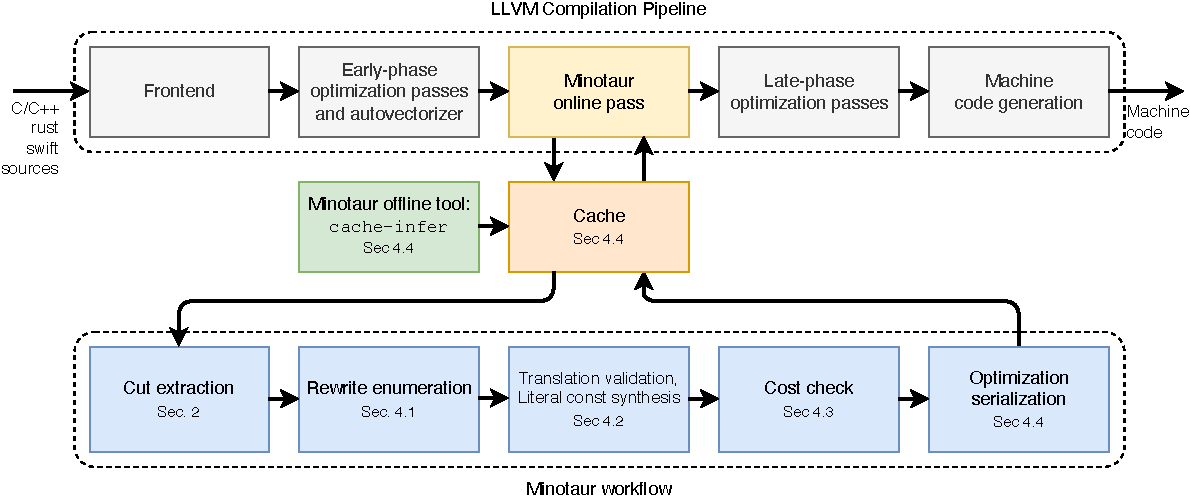
\includegraphics[width=\linewidth]{figures/flowchart.pdf}
     \caption{Overview of how \minotaur{} works, and how it fits into the
       LLVM optimization pipeline}
     \label{fig:workflow}
\end{figure}

Figure~\ref{fig:workflow} illustrates \minotaur's high-level structure,
and how it fits into LLVM\@.
%
It works by extracting many different \textit{cuts} from an LLVM function.
%
Each cut serves as the specification for a program synthesis
problem, where the objective is to synthesize a new cut that refines
the old one and is cheaper.
%
When such a cut is found, \minotaur{} uses it to rewrite the original
LLVM function, and also caches the rewrite.


Reasoning about the correctness of optimizations at the level of LLVM
IR can be very difficult; I have repurposed Alive2~\cite{alive2} to
serve as a verification backend.
%
To Alive2, I added formal semantics for 165
Intel-architecture-specific SIMD intrinsics.
%
Reasoning about the relative costs of code sequences is another
difficult problem; the solution adopted by \minotaur{} is to reuse the
LLVM Machine Code Analyzer~\cite{llvmmca}, which has adequately
accurate pipline models for various modern processors.
%
These tools, along with the LLVM compiler itself, form the
foundation upon which \minotaur{} is built.


\textbf{Research contributions:}
%
First, I designed and implemented a domain-specific program
transformer that extracts an SSA value from an LLVM function, along
with context about how that value was computed.
%
Extracting enough context to permit interesting optimizations, without
extracting so much context that the underlying SMT solver was
overwhelmed, was an interesting empirical problem.
%
Second, I created a synthesis engine that searches for cheaper code
sequences; it enumerates partially symbolic candidates where the
instructions are concrete, but data values are symbolic.
%
Third, I developed infrastructure for caching optimizations and also
for applying them to code that is being compiled.
%
All together, these elements run inside of an LLVM optimization pass.
%
Finally, I performed a detailed evaluation of \minotaur's ability to
speed up code, showing that it can find numerous optimziations that
LLVM fails to perform, and also that it can achieve speedups on a
variety of real-world libraries and benchmarks.

